\section{Coding Theory Fundamentals}

Before proceeding we need to build a framework of definitions and the general idea behind Coding Theory. This paper is designed such that anyone with a basic background in mathematics can understand. The details of what information and entropy are have been moved under the section 'Shannon's Theorem' for convenience as they follow directly into his idea of relating channel capacity with information rate of a code. \\

In real life, messages are sent as a block of symbols through some medium, aka a 'channel'. For example, binary code. \\

\textbf{Channel:} a formal mathematical model of communication that operates abstractly like a function, in the sense that it has input and output sets. Channels apply a probabilistic function on each symbol of the input to produce the output. The set of all symbols is the alphabet $\Sigma$\\

In our case we use the Binary Symmetric Channel.

\textbf{Binary Symmetric Channel (BSC):} both input and output sets consist of the alphabet $\Sigma = \{1, 0\}$. The probabalistic function is the Bernoulli random variable with probability $p$ of being flipped as visualised in Figure \ref{fig:bsc} and Equation \ref{eqn:bsc}. The Bernoulli random variable is hereafter denoted as as $X \sim Bern(p)$.





\begin{equation}
\label{eqn:bsc}
    u =  \begin{cases} 
      u & 1-p \\
      u' & p 
\end{cases}
\end{equation}

\begin{figure}
    \centering
    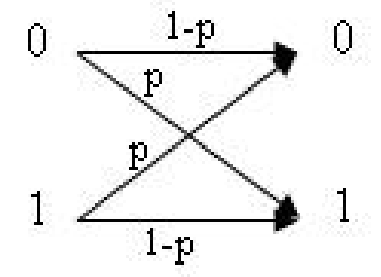
\includegraphics[width=0.5\linewidth]{images/bsc.png}
    \caption{Model of a $BSC_p$}
    \label{fig:bsc}
\end{figure}

A more generalized channel is also the discrete memoryless channel. However, we will not be discussing it in this paper.
\textbf{Discrete Memoryless Channel:} Channels that transmit sets of symbols from a finite alphabet $\Sigma$. \emph{Memoryless} simply means that the probabilistic function is independent of messages sent before the current message. \\



Now that errors have been modeled, we must find a way to correct or detect them. Here we introduce the notion of codes through the below definitions. \\

\textbf{error-correcting code:} an algorithm that represents messages of length $k$ as codewords of length $n$ where $n > k$ such that the occurance of errors after transmission can be detected or corrected. \\

\textbf{message:} a sequence of symbols $\textbf{u} = u_1u_2 ... u_k$. It is the information we desire to transmit. \\

\textbf{codeword:} A sequence of symbols $\textbf{x} = x_1x_2...x_n$ where each codeword corresponds directly to a message \textbf{u} as $\textbf{x} = \textbf{x}(\textbf{u}).$ \\

The set of all messages and codewords are $U$ and $\chi$, where $|\chi| = |U| = 2^k$ \\

More specifically, we are looking at Linear Codes, the parent family of Polar Codes. \\

\subsection{Definitions and Properties of linear codes}

\vdent

\textbf{Definition 1:} A code is linear if there exists a matrix $H$ such that $Hx^T = 0 \ \ \ \ \forall u$. This is called the parity check matrix.  \\

    (a) Additionally, $H(x+y)^T = Hx^T + Hy^T = 0$ and so $x+y$ is also considered a codeword. This is the linearity property of linear codes.\\


\textbf{Definition 2:} For every linear code there exists a $k \text{ x } n$ generator matrix $G$ such that $\textbf{x} = \textbf{u}G$ and $GH^T = HG^T = 0$. \\

\textbf{Definition 3:} The information rate (or efficiency) of a code is $R = \frac{k}{n}$. \\

The matrices and properties above can be used directly to encode and decode simple codes via the H and G matrix pair.

\textbf{Definition 4:} The Hamming weight is the count of '1's present in a base 2 vector. It is denoted by $wt(\textbf{x})$ \\

\textbf{Definition 5:} The Hamming distance between any 2 vectors $\textbf{x}$ and $\textbf{y}$ is defined as the number of differences between them. The notation is as follows: $dist(\textbf{x}, \textbf{y)} = wt(\textbf{x} - \textbf{y})$ \\

\textbf{Definition 6:} The minimum distance of a code is the minimum Hamming distance between any two codewords. It is often parameterized as $d$. This is simply referred to as the \emph{distance} of a code.  \\

\textbf{Definition 7:} the XOR operation between any two bits is denoted X + Y where X and Y are bits, and is defined in Figure \ref{fig:xor} \\

\begin{figure}
    \centering
    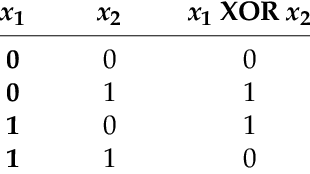
\includegraphics[width=0.5\linewidth]{images/xor.png}
    \caption{XOR truth table}
    \label{fig:xor}
\end{figure}

Finally, we can describe simple binary codes as a set of parameters $[n, k, d]$, encapsulating the message and codewords size, alongside the minimum distance between each codeword.

To better understand the minimum hamming distance of a code, recall that the size of the set of codewords and messages are equal, yet the length of each codeword is longer than the original message. This means the set of codewords $\chi \subset {\{0,1\}^k}$, leaving gaps in between.

We can visualize this using Hamming balls in Figure \ref{fig:balls}. The center represents a valid codeword and the radius outlines the area containing other elements of ${\{0,1\}^k}$ that aren't codewords. These are the elements obtained due to some error during transmission. 

\begin{figure}[H]
    \centering
    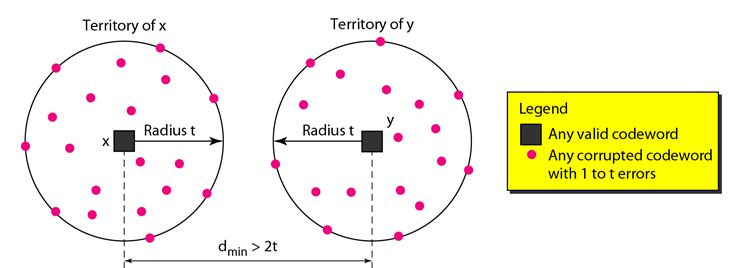
\includegraphics[width=0.75\linewidth]{images/hammingball.jpg}
    \caption{Visualization of Hamming balls with radius t and minimum distance of 2t. x and y are both codewords}
    \label{fig:balls}
\end{figure}


Encoding is a simple process of just applying the generator matrix. We now explore one simple decoding method that will also provide insight into what the minimum distance truly means and its importance in maintaining a stable code.

\subsection{Minimum distance decoding}

Given a codeword $x$ sent over a BSC such that the received codeword is $y$ and probability of error is $0 \le p < \frac{1}{2}$, the error vector is $e = x-y$. It describes the differences between sent and received codewords. The number of errors, aka the weight of e, is denoted $a$. In an ideal case, for example, $e$ would be a zeros vector with $a = 0$ . 

We can find the probability of each error as $Pr(e = w) = p^a(1-p)^{n-a}$. Where $w$ is some error vector.\\

By observing the pattern as $a$ increases, we see that the most probable error vector (that is non-zero) is one with the least number of errors.
As $(1-p)^n > p(1-p)^{n-1} > p^2(1-p)^{n-2} > \dots$ due to our bounds on $p$, we can see that the most probable error vector (that is non-zero) is one with the least number of errors. Using this, we can test all $2^k$ error vectors in order from smallest to greatest error until we find a value for $x$ that is within the set of all valid codewords $\chi$.

In minimum distance decoding, the radius of the hamming ball is the maximum number of errors that can occur and still be corrected. If there is an overlap between hamming balls, then there is the possibility of an error occurring where it could be corrected to either valid codeword. By introducing redundancy, we increase the minimum distance to reduce this overlap, but as a result reduce the efficiency of the code.


For example, take codewords $c_1$ and $c_2$. if the distance between them is 1, we can only detect an error of distance 1 using the parity matrix, but cannot correct it with certainty. This is because we cannot determine which codeword the error originated from. However, if we have a distance of 2, we can detect errors up to distance 2 and we can correct error up to a distance of 1. This can be visualized as hamming balls with a distance between codewords of 2, and radius of 1, resulting in no overlap and is thus stable.

\subsection{Extra Mathematics}

The following mathematical ideas will help in our understanding of Shannon's Theorem but are not essential for the paper.

\subsubsection{Law of Large Numbers (LLN)}

The LLN states that as the sample size (n) of a random variable increases, the sample mean converges to the expected value (population mean).

Let $X_1, X_2, \dots, X_n$ be independent and identically distributed (i.i.d.) random variables
with finite mean $\mu = \mathbb{E}[X_i]$. The average is

\[
\overline{X}_n = \frac{1}{n} \sum_{i=1}^n X_i.
\]


Weak Law of Large Numbers: For any $\epsilon > 0$,
    \[
    \Pr\left( \, \big| \overline{X}_n - \mu \big| > \epsilon \, \right) \to 0
    \quad \text{as } n \to \infty.
    \]
    This means that the sample average converges to $\mu$ in probability.

\subsubsection{Chernoff Bounds}

Chernoff bounds help us find the probability of obtaining a large value in a  random variable. 

Imagine you are flipping a biased coin $n$ times. You expect to see $np$ heads, but in reality it could be within some range of $np$. 

Chernoff bounds state that the probability of obtaining a value far from $np$ decreases exponentially as $n$ increases. 

This is different from the Law of Large numbers, which would instead state that the fraction of heads to tails would approach $p$.


This probability is formally defined as:

\[P(X \ge a) \le e^{-at}M_x(t)\: \ \ \ \ \forall t > 0\]
Where $M_x(t)$ is the Moment Generating Function and $a = (1+\delta)\mu$ as seen in \ref{fig:chernoff}.
\begin{figure}[h]
    \centering
    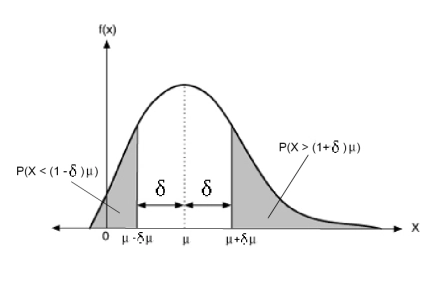
\includegraphics[width=0.5\linewidth]{images/chernoff.png}
    \caption{Probability distribution of a random variable}
    \label{fig:chernoff}
\end{figure}

